\section{Обзор предметной области}
\label{sec:domain:intro}

В данном разделе будет произведён обзор программых средств аналогичных разрабатываемому в рамках дипломного проекта - определение психологических параметров человека по образцу почерка, а так же литературных источников. Проанализированны преимущества и недостатки различных подходов к выделению и классификации признаков рукописного текста.

\subsection{Графология}
\label{sub:domain:grafologic}
\emph{Графология} - это учение, постулирующее наличие устойчивой связи месту почерком и индивидуальными особенностями личности.

Идея использования почерка для выявления психологических параметров личности впервые была предложена в 1622 в книге итальянского профессора Камилло Бальдо "Как узнать природу и качества человека, взглянув на букву, которую он написал"~\cite{kamillo_grafology}. Первым кто систематизировал знания стал Фландрэна аббат Мишон в 1872 году. Он проанализировал большое количество работ по графологии и образцов почерка и в своей книге "Систeмa графологии" предложил \emph{метод Мишона}, он основывался на анализе штрихов, букв, слов, свободных движений, строк и пр.~\cite{mishon_grafology}

Начиная с середины 20 века графология начала рассматриваться как псевдонаучное учение. По результатам исследования профессионалльным графологам не удалось достоверно оценить трудовые способности человека. В среднем профессиональные графологи давали такую же по степени достоверности оценку, как и люди «с улицы»~\cite{neter_shakhar_psevdograph}~\cite{neter_shakhar_psevdograph}. В десятках исследований было показано отсутствие связи особенностей почерка с трудовыми способностями человека.

Тем не менее графология широко используется в современной практике отбора кадров.

Основные признаки почерка, которые анализирует графологическая экспертиза:
\begin{enumerate}
  \item Размер букв (очень маленькие, маленькие, средние, крупные);
  \item Наклон букв (левый наклон, легкий наклон влево, правый наклон, резкий наклон вправо);
  \item Направление почерка: (строчки ползут вверх, строчки прямые,  строчки ползут вниз);
  \item Размашистость и сила нажима: (легкая, средняя, сильная, очень сильная);
  \item Характер написания слов: (склонность к соединению букв и слов, склонность к отдалению букв друг от друга, смешанный стиль);
  \item Общая оценка: (почерк старательный, почерк неровный, почерк небрежный, почерк неразборчивый).
\end{enumerate}

Перечисленные параметры почерка являются устойчивыми, но все же присутсвует естественные отклонения параметров (длина, ширина, толщина, угол) от средних значений. Вариация становится наиболее заметной при изменение психоогического состояния человека, например при страхе, беспокойстве, алкогольном опъянении.

\subsection{Анализ аналогов}
\label{sub:domain:analogs}

\subsubsection{ScriptAlyzeR}
\label{sub:domain:analogs:neuro_script} 


Программое средство "ScriptAlyzeR" является частью семейства программых средств для работы с рукописным текстов компании "NeuroScript" и представляет собой декстопное приложение для операционных систем Windows.

\begin{figure}[ht]
    \centering
    \label{fig:domain:analogs:neuro_script}
    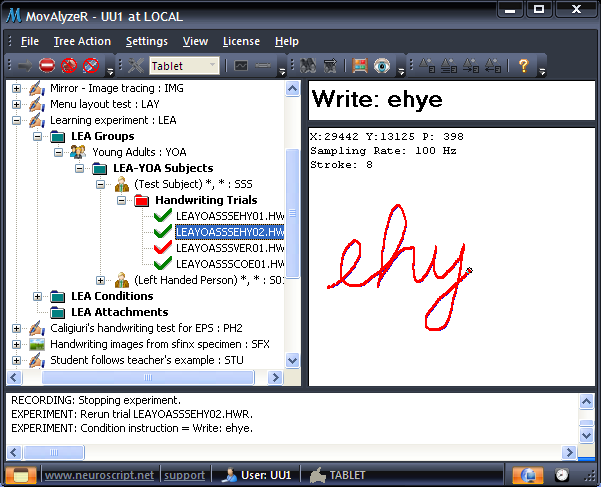
\includegraphics[width=0.7\textwidth]{neuroscript.png}
    \caption{Программое средство "ScriptAlyzeR"}
\end{figure}

Основными возможностями ПС являются:
\begin{itemize}
	\item Мультимодальные движения. Положение ручки, давление, ориентация, положение мыши и положение пальца на 100-200 Гц.
	\item Бимануальные движения. Измеряйте координацию, записывая одновременно две ручки.
	\item Real-Time, Real-Size Обратная связь. Для планшетных компьютеров и планшетов. Отображение и печать в реальном размере.
	\item Изменение толщины линии. Непосредственная визуальная и звуковая обратная связь с пером.
	\item Искаженная визуальная обратная связь. Поворот, перекос и отражение на мониторе компьютера в режиме реального времени.
	\item Моделирование. Генерировать рукописные цифровые данные с шумом с известными характеристиками штрихов для проверки точности обработки.
	\item Проверка непротиворечивости. Проверяйте каждое испытание, когда оно записано.
	\item Знание результатов. Покажите участникам, насколько хорошо они после каждого испытания показали максимальную производительность и стабильность.
	\item Многостраничные записи. Разделить текст на слова и штрихи.
	\item Внешние приложения. Полная интеграция с вашими собственными модулями с использованием сценариев MATLAB® или скомпилированных программ.
	\item Оптически сканированные изображения. Сегмент в визуальные штрихи и оценка характеристик за такт.
	\item Изображение для движения. Сканируйте Архимеды спиралями из бумаги и проанализируйте их как последовательность движения.
\end{itemize}


\subsubsection{PUF на интегральных микросхемах. }
\label{sub:domain:puf_physical_types:ic}

Аналогично пузырькам в оптической системе, в иных средах тоже можно получить неклонируемость. Рассмотрим среду, и так широко используемую в цифровых устройствах - электрические проводники и диэлектрики.
Любое современное технологичное устройство содержит в себе внушительное количество интегральных микросхем. На них и построены PUF данного типа. Несмотря на то, что микросхемы изготавливаются по одному и тому же технологическому процессу, каждая из них достаточно уникальна для корректной работы PUF. Это может быть использовано в системах информационной безопасности как уникальный идентификационный признак устройства.

Один из вариантов построения такой PUF: интегральная микросхема покрывается слоем защитного вещества со вкраплениями диэлектрика. Эти вкрапления имеют случайные размер и форму. Под этот слой подводятся электроды"=датчики. В совокупности с защитным слоем каждый такой электрод обретает свойства конденсатора случайной (зависящей от вкраплений диэлектрика в защитный слой) ёмкости. Очевидно, что случайность ёмкости каждого конденсатора достигается при размере частиц, сравнимом с размером между электродами.


\subsubsection{PUF на полевых транзисторах. }
\label{sub:domain:puf_physical_types:transistors}

В основе таких PUF лежит особенность полевых транзисторов задерживать сигнал, проходящий по нему на непредсказуемое время, зависящее от физических свойств материала транзистора (именно из"=за материала такие PUF ещё называют кремниевыми). Физическая система PUF будет состоять из набора пар транзисторов и триггеров"=арбитров. Триггер будет давать на выход 0 или 1 в зависимости от того, сигнал с какого из пары транзисторов пришёл к нему раньше. Подавая на вход этому набору некоторый сигнал"=запрос, на выходе исследователь получит набор значений триггеров - реакцию системы на запрос, уникальную для данного устройства, в состав которого включаются упомянутые транзисторы.

Неклонируемость строится на физической неидеальности процесса производства. Изучение функции для последующего математического прогноза реакции на запрос возможно только полным перебором входных сигналов, что является достаточно вычислительно сложной задачей.


\subsubsection{PUF на магнитных элементах. }
\label{sub:domain:puf_physical_types:magnetic}

Практическое применение - уникальный идентификатор магнитной полосы банковской карты. Частицы феррита бария, содержащиеся в пасте"=основе магнитной полосы, также имеют случайный размер и форму. Логично сделать вывод, что на случайности их распределения можно построить PUF. Неклонируемость снова опирается на физическую неидеальность процесса производства. Неточности и погрешности не дадут повторить рисунок частиц феррита бария в  точности. А математическое моделирование не препятствует выполнению данной PUF её задачи.
\begin{figure}[ht]
    \centering
    \label{fig:domain:puf_physical_types:magnetic}
    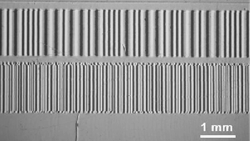
\includegraphics[width=0.55\textwidth]{magneticstripe.png}
    \caption{структура магнитной полосы -- варианта магнитной PUF}
\end{figure}

\subsection{Виды PUF по принципу работы. }
\label{sub:domain:puf_types}


\subsubsection{PUF типа арбитр (Arbiter PUF). }
\label{sub:domain:puf_types:arbiter}

Физически неклонируемые функции по типу арбитра - разновидность физически неклонируемых функций на основе задержек. Идея состоит в том, чтобы привнести состояние гонки между двумя путями микросхемы. Оба пути заканчиваются элементом"=арбитром, который определяет какой из путей был быстрее и выдает соответствующее бинарное значение.
\begin{figure}[ht]
    \centering
    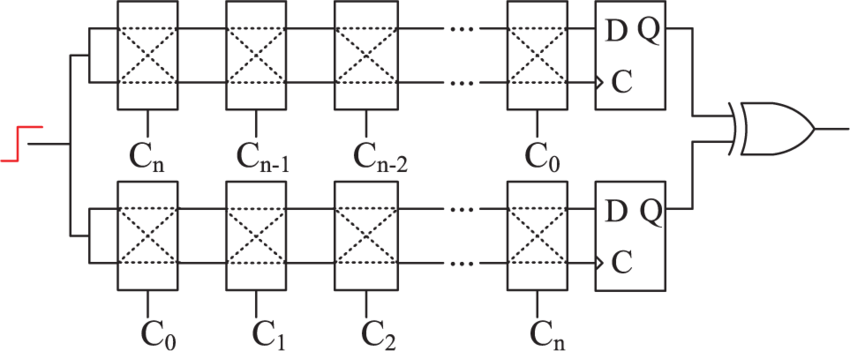
\includegraphics[width=0.7\textwidth]{arbiter.png}
    \caption{PUF типа арбитр}
    \label{fig:domain:puf_types:arbiter}
\end{figure}

Основная идея реализации этого типа PUF состоит в построении двух идентичных путей сигнала на одном кристалле интегральной схемы. Такие пути называются симметричными и имеют очень близкие по значению длины и промежутки времени распространения сигнала. Однако, они не являются полностью идентичными ввиду различных задержек $d$ на каждом отрезке пути, обусловленными вариацией техпроцесса. Измерение различий во времени пути сигнала осуществляется с помощью одновременной подачи сигналов на входы симметричных путей и регистрации моментов получения сигналов на выходах каждого из путей. Симметричные пути проектируются в виде конфигурируемых соеднений на основе мультиплексоров, управляя количеством которых, а также сигналами, подаваемыми на управляющие их входы, можно создавать различные комбинации путей прохождения сигнала. Для сравнения симметричных путей применяется арбитр -- элемент, значение на выходе которого определяется тем, по какому пути сигнал достиг его раньше. Простейший вариант арбитра - синхронный D-триггер. Схема такого построения PUF показана на рисунке~\ref{fig:domain:puf_types:arbiter}.

Таким образом, в качестве битов запроса $C_i \in \{0,1\} $ принимаются сигналы управляющих входов мультиплексоров, а выходным значением $R_i$ будет являться сигнал на выходе элемента-арбитра, к входам которого подключены выходы симметричных путей. Возможна также другая реализация, где вместо мультиплексоров используются трёхстабильные буферы. PUF типа арбитр на трёхстабильных буферах потребляет значительно меньше энергии при меньшей площади кристалла.

\subsubsection{PUF на базе кольцевого генератора (RO"=PUF). }
\label{sub:domain:puf_types:ring_oscillator}

Физически неклонируемые функции на базе кольцевых генераторов также используют неконтролируемые изменения задержек процессов цифровых компонентов в качестве источника случайности. Когда эти компоненты образуют кольцевой генератор, частоты его выходных сигналов различаются, что и используется при формировании бинарного ответа.

\begin{figure}[ht]
    \centering
    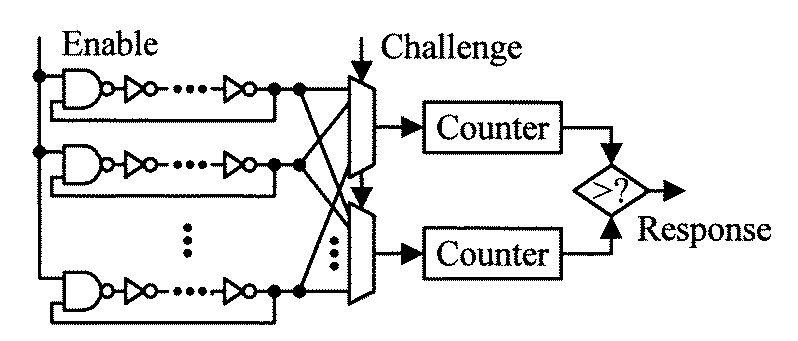
\includegraphics[width=0.8\textwidth]{ro-puf.png}
    \caption{PUF на базе кольцевого генератора}
    \label{fig:domain:puf_types:ring_oscillator}
\end{figure}

Данный тип физически неклонируемой функции основан на использовании частотных характеристик кольцевых генераторов, представляющих собой схемы из подключенных инверторов с отрицательной обратной связью. Число инверторов в цепи должно быть нечётным для обеспечения получения, выходного сигнала в виде меандра, частота которого как раз и определяется задержкой распространения обратного сигнала. Схема кольцевого генератора показана на рисунке~\ref{fig:domain:puf_types:ring_oscillator}.

Для обеспечения стабильного состояния каждый генератор дополнен элементом элементом \emph{И} на входе. Управление ФНФ на основе кольцевого генератора осуществляется путём подачи вектора входных сигналов $C_i$ на управляющие входы мультиплексоров, подсоединённых к выходам кольцевых генераторов. Основой формирования ответа $R_i$ является результат сравнения частот генераторов. Таким образом, набор генераторов будет имет произвольное соотношение частот и уникально характиризовать устройство, в котором они реализованы.

\subsubsection{PUF на базе статического ОЗУ (SRAM PUF). }
\label{sub:domain:puf_types:sram}
Стати
Принцип работы физически неклонируемых функций на базе статического оперативного запоминающего устройства (СОЗУ) основан на случайности состояния части ячеек СОЗУ при включении.

\begin{figure}[ht]
    \centering
    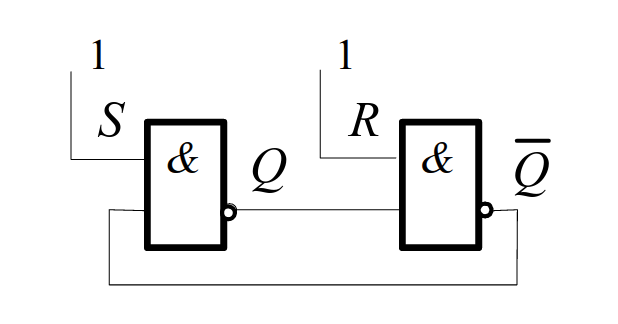
\includegraphics[width=0.76\textwidth]{rs_sram.png}
    \caption{PUF на базе ячейки статического ОЗУ в виде RS-триггера}
    \label{fig:domain:puf_types:sram}
\end{figure}

Статические оперативные запоминающие устройства (СОЗУ) широко используются в вычислительной технике для хранения данных. Непосредственно запоминающий элемент СОЗУ (ячейка) состоит из четырех транзисторов, реализующих два инвертора с перекрестными обратными с связями. Подобная ячейка всегда находится в одном из двух состояний, что, в свою очередь, позволяет использовать ее для хранения одного бита информации. Примером такой ячейки может служить RS-триггер, реализованный на двух логических элементах \emph{2И-НЕ}, представленный на рисунке~\ref{fig:domain:puf_types:sram}. Высокий уровень сигнала (логическая единица), подаваемый одновременно на оба входа RS-триггера, позволяет сохранять предыдущее состояние. При включении питающего напряжения все ячейки СОЗУ устанавливаются в одно из двух возможных состояний -- 0 или 1; причем в силу симметрии RS-триггера априори неизвестно, какое конечное состояние примет ячейка. Экспериментально подтверждено, что большинство ячеек СОЗУ при включении питающего напряжения преимущественно переходят в одно из двух состояний. Причиной этого является несимметричность прямых и обратных связей RS-триггера, обусловленная особенностями технологии изготовления.


\subsubsection{PUF типа <<бабочка>> (Butterfly PUF). }
\label{sub:domain:puf_types:butterfly}
Физически неклонируемые функции по типу бабочки имитирует работу ячейки СОЗУ, формируя перекрестные обратные связи для получения бистабильной схемы. В отличие от ФНФ на базе ячейки СОЗУ, данная функция состоит из двух асинхронных D-триггеров. Схема принудительно переводится в неустойчивое состояние путем подачи взаимоюсключающих сигналов на входы триггеров, после чего схема переходит в одно из двух стабильных состояний, которое зависит от случайной разности задержек в паре линий обратной связи и линии входного сигнала~\cite{yarmolik_vashinko}. Своё название данная разновидность получила благодаря виду схемы, на которой она реализована.
\begin{figure}[ht]
    \centering
    \label{fig:domain:puf_types:butterfly}
    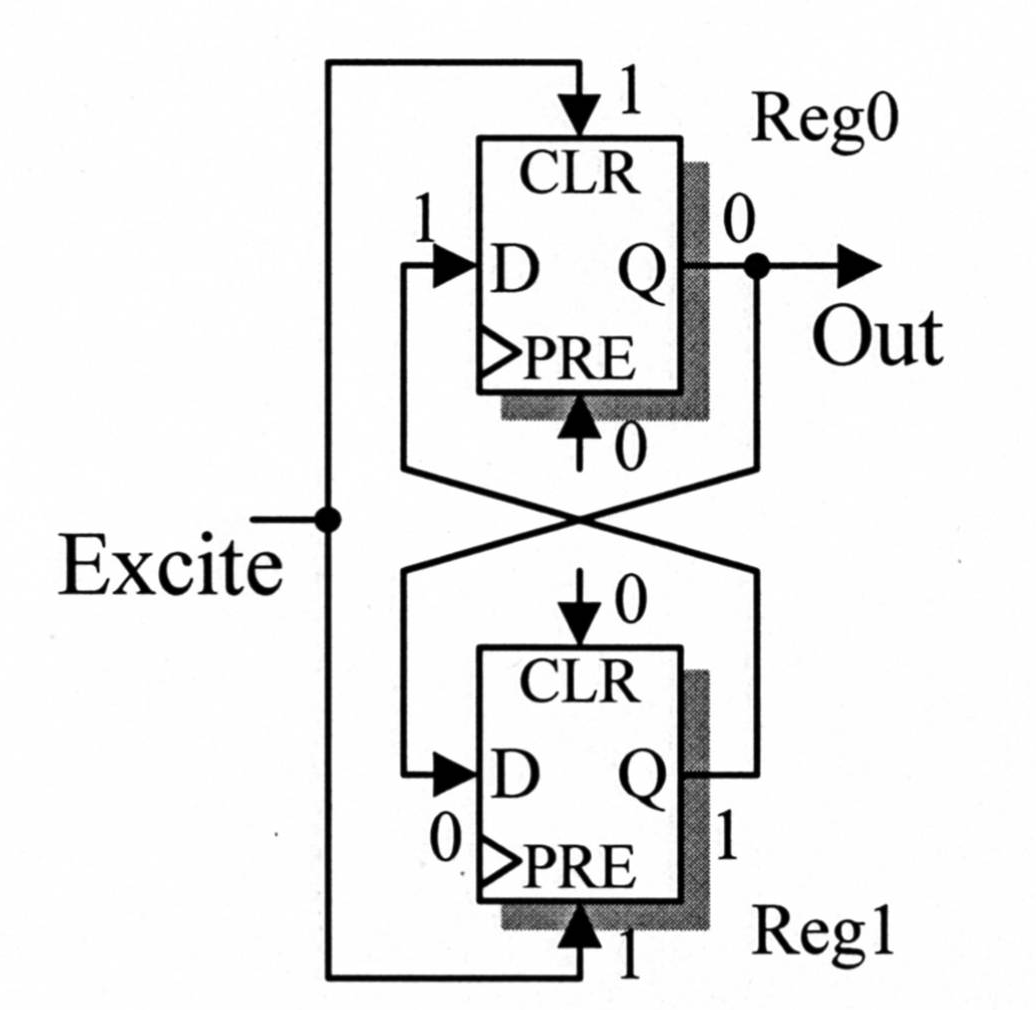
\includegraphics[width=0.6\textwidth]{butterfly.png}
    \caption{PUF типа <<бабочка>>}
\end{figure}


\subsubsection{PUF на основе сбоев (Failure PUF). }
\label{sub:domain:puf_types:failure_puf}

Этот тип физически неклонируемых функций основываются на сбоях в поведении комбинаторных логических схем. В идеале у комбинаторной схемы нет внутреннего состояния, что означает, что стационарный выход полностью определяется его входными сигналами. Однако, когда логическое значение на входе изменяется, для достижения стационарного значения на выходе требуется некоторое время. Появление сбоя определяется различиями в задержках различных логических цепей от входов к выходному сигналу. Так как задержки определенных образцов комбинаторных схем вызваны случайными изменениями процесса, появление, количество и форма сбоев выходных сигналов также будут случайными и характерными для определенных образцов схемы. Поэтому оценка поведения сбоев таких схем может быть использована для ответа физически неклонируемой функции.

Стоит заметить, что в данном списке перечислены лишь базовые варианты реализации PUF. На их основе и на основе комбинаций этих типов может быть построено огромное множество различных сложных PUF~\cite{cryptowiki_pufs, rmaes_pufs}.


\subsection{Использование PUF для идентификации и аутентификации цифровых устройств}
\label{sub:domain:puf_auth}
Аутентификация традиционно характеризуется как процесс проверки того, что сущность владеет конкретной информацией, например, паролем, обладает конкретными свойствами, или же является именно тем, за что себя выдает. Многофакторная аутентификация представляет собой комбинацию этих проверок. Аутентификация на основе физически неклонируемых функций подразумевает наличие разных независимых устройств, каждое из которых характеризуется набором паролей (т.е. в данном случае -- набором пар запрос"=ответ), который однозначно идентифицирует эти устройства, то есть, в какой-то степени, аутентификацию на основе PUF можно считать многофакторным механизмом.

Множество возможных применений ФНФ также включает шифрование информации, обнаружение вредоносных изменений структуры интегральной микросхемы, контроль специфических функций устройств и многие другие. Каждый из сценариев использования предъявляет определенные требования к свойствам используемой ФНФ. В частности, для использования в криптографических целях, ФНФ должна быть устойчива к атакам моделирования, т.е. должна препятствовать построению более-менее точной модели своей структуры и/или поведения. Это же применимо и к протоколам аутентификации на основе ФНФ. Общее правило -- чем больше контроля над своими входными и выходными параметрами ФНФ предоставляет приложению, тем лучше оно должно быть защищено от таких атак.

Применительно к аутентификации на основе ФНФ применяют термины \emph{электронный ключ (токен)} -- для обозначения утройства, оснащённого ФНФ, чья подлинность проверяется, например, смарт-карта или RFID-метка~\cite{rfid_puf}, и \emph{доверенный сервер} -- для обозначения стороны, располагающей истинными данными идентификации конкретных устройств.

Существует два основных подхода к осуществлению системы аутентификации, основанной на физически неклонируемых функциях. Первый подход состоит в получении стойкого и безопасного криптографического ключа из ответа физически неклонируемой функции и использовании этого ключа в каком"=либо из протоколов аутентификации. В этом случае ФНФ используется в качестве или как составная часть генератора истинно случайных чисел с показателями, достаточными для его применения в криптографических целях. Секретность ключа повышается тем, что в открытом виде могут храниться только данные, использованые для его генерации, в данном случае -- наборы пар $\crp$. Следовательно, воспроизвести ключ возможно только при использовании исходной ФНФ и с данным набором входных данных. Для этого подхода достаточно довольно простой ФНФ (т.н. \emph{weak PUF, слабая ФНФ}), способной сгенерировать достаточное для построения ключа количество случайной информации, но при этом устройство должно содержать реализацию криптографического алгоритма, чтобы из входного набора сконструировать ключ. К сожалению, этот метод уязвим к атаке по стороннему каналу (\emph{side-channel attack}): злоумышленник может получить секретный ключ, используя уязвимости в аппаратной реализации алгоритма~\cite{pufbased_auth,puf_cryptography}.

Другой подход состоит в разработке схемы аутентификации, которая напрямую применяет уникальность и непредсказуемость поведения пары запроса"=ответа отдельного объекта. Такая схема состоит из двух фаз (регистрации в системе и подтверждения подлинности).

В первой фазе, каждый объект проходит регистрацию у проверяющего. Во время этой фазы проверяющий записывает идентификатор каждого объекта и собирает значительное подмножество пар запрос"=ответ каждого объекта (устройства) для случайно сгенерированных запросов. Собранные пары запрос"=ответ хранятся в базе данных проверяющего.

Во время фазы подтверждения, объект (устройство) посылает проверяющему свой идентификатор. Проверяющий находит его в базе данных, выбирает оттуда случайную пару запрос"=ответ, которая соответствует полученному идентификатору. Запрос посылается объекту, объект вычисляет физически неклонируемую функцию и посылает ответ. Проверяющий сравнивает этот ответ со значением из базы данных, и если проверка прошла успешно, тообъект аутентифицирован, иначе -- аутентификация отклонена. Использованная пара запрос"=ответ удаляется из базы данных для исключения возможности сохранения результатов третьей стороной. Корректность данной схемы аутентификации обеспечивается тем фактом, что ответы физически неклонируемых функций воспроизводимы самим объектом в течение долгого времени.
Однако, подход в описанном выше виде имеет существенные минусы:
\begin{itemize}
  \item Число возможных пар $ \crp $ может быть, а в реальных PUF почти всегда является очень большим. Вследствие этого, регистрация устройства путем сбора достаточного для последуещей аутентификации количества пар не всегда возможно за приемлемое время.
  \item Несмотря на то, что ответы физически неклонируемых функций воспроизводимы самим объектом, ФНФ редко являются полностью стабильными. Подавляющее большинство реализаций имеют дополнительную зависимость выходного сигнала от побочных эффектов, таких как физический износ устройства, температура окружающей среды, влажность и других параметров. В связи с этим, однозначное соответствие нескольких выходных сигналов $ R $, вызванных одним набором $ C $, не может быть гарантировано.
\end{itemize}

Из-за этих нюансов, использование <<наивной>> реализации протокола не представляет особой практической ценности. Поэтому данный дипломный проект ставит целью исследование и реализацию усовершенствованного протокола аутентификации, учитывающего указанные особенности и предоставлящего достаточный уровень секретности и защиты от перехвата данных или управления третьей стороной.


\subsection{Обзор существующих аналогов}
Подавляющее большинство средств защиты интеллектуальной собственности применительно к цифровым устройствам, в частности, программные средства аутентификации устройств на основе физически неклонируемых функций, а также особенности их реализации сами по себе являются коммерческой тайной. В связи с этим, даже поверхностный анализ и сравнение существующих аналогов не представляется возможным. Однако, целесообразным представляется создание доступного открытого аналога средства аутентификации, которое, в противовес проприетарным решениям компаний"=производителей, могло бы служить удобной базой для дальнейшей развития и затачивания под конкретные нужды энтузиастами разработки цифровых устройств, а также в образовательных целях.


\subsection{Постановка задачи}
В результате выполнения дипломного проекта должно быть разработано программное средство аутентификации цифровых устройств, реализующее протокол взаимодействия между сервером аутентификации и цифровым устройством, включающим в себя некоторую реализацию PUF для однозначной его идентификации. К разрабатываемому программному средству предъявляются следующие требования:
\begin{itemize}
\item разрабатываемое ПО должно работать на операционных системах Linux, MacOS и Windows;
\item программное средство должно быть выполнено в виде клиент"=серверного приложения;
\item программное средство должно поддерживать работу как в режиме выделения признаков рукописного текста, так и в режиме их классификации;
\item программное срелство должно предусматривать механизм регистрации, аутентификации и авторизации пользователей.
\end{itemize}
